\item
\mbox{}
\begin{center}
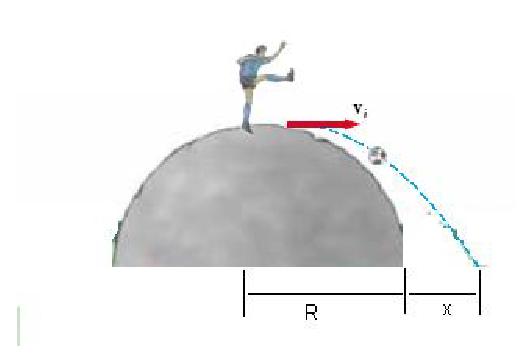
\includegraphics [scale=0.7]{latex/eps/1_4_2_image_1.eps}
%\caption{Gambar orang menendang bola}
\end{center}
Seseorang berdiri pada batu setengah bola yang beradius R menendang bola, sehingga bola mempunyai kecepatan horizontal $v$. \\ a$)$ Berapa kecepatan awal bola, jika bola tidak pernah menyentuh batu tersebut. \\
b$)$ Dengan kecepatan kritis(kecepatan dimana bola hampir menyentuh bola), berapa jauhkan bola itu jatuh ke tanah terhadap batu.

\begin{description}
\item[Solusi:]
Pada gerak parabola yg berada ketinggian $R$ berlaku $x=v t$ dan $y= R-\frac{1}{2}g t^{2}$.\\ \\
jadi 
	\[y=R-\frac{1}{2 v^{2}} g x^{2}
\]
a. Jika bola berada pada batu, maka ketinggian bola ($y_{batu}$), memenuhi
	\[y^{2}_{batu} +x^{2}=R^{2}
\]
Pada $x=0$ maka $y=y_{batu}$. Dan syarat bola tidak menyentuh batu yaitu $y \ge y_{batu} $, jadi
\begin{eqnarray*}
y \ge y_{batu} \\
y^{2} \ge y^{2}_{batu} \\
y^{2} \ge -x^{2} + R^{2} \\
y^{2} +x^2 \ge R^{2} \\
\big(R-\frac{1}{2 v^{2}} g x^{2}\big)^{2} + x^{2} \ge R^{2} \\
R^{2} -\frac{g x^{2} R}{2 v^{2}}+ \frac{g^{2} x^{4} R^{2}}{4 v^{4}} +x^{2} \ge R^{2} \\
\frac{g^{2} x^{4} R^{2}}{4 v^{4}} +x^{2} \ge \frac{g x^{2} R}{2 v^{2}} \\
\frac{g^{2} x^{2} R^{2}}{4 v^{4}} +1 \ge \frac{g  R}{2 v^{2}}
\end{eqnarray*}
Jika pertidaksamaan tersebut berlaku untuk $x$ mendekati nol, maka syarat $y^{2}_{batu} +x^{2}=R^{2}$ terpenuhi untuk semua $x$. Jika lintasan bola sejak awal mempunyai jari-jari kelengkungan yang besar, maka bola tidak akan menyentuh batu selama di lintasan.\\
Dengan mengambil $x$ mendekati nol pada pertidaksamaan diatas, menjadi
\begin{eqnarray*}
	\lim_{x\rightarrow 0} \big(\frac{g^{2} x^{2} R^{2}}{4 v^{4}} +1\big) &\ge& \lim_{x\rightarrow 0} \big(\frac{g  R}{2 v^{2}} \big) \\
	1 &\ge& \frac{g  R}{2 v^{2}} \\
	v &\ge& \sqrt{g R}
\end{eqnarray*}
Kesimpulannya, bola tidak akan menyentuh batu bila $v$ memenuhi
\begin{equation*}
v \ge \sqrt{g R}
\end{equation*}  

b)Kecepatan kritis yaitu pada $v = \sqrt{g R}$.\\
Menggunakan persamaan ketinggian bola, yaitu
\begin{eqnarray*}
y&=&R-\frac{1}{2 v^{2}} g x^{2} \quad \textrm{substitusi} \,v=\sqrt{g R}, \textrm{menjadi} \\
y&=&R-\frac{1}{2 g R} g x^{2} \quad \textrm{syarat bola menyentuh tanah jika} \, y=0 \\
0&=&R-\frac{1}{2 g R} g x^{2} \\
x&=&R\sqrt{2}
\end{eqnarray*}
Jarak dari bola yaitu, 
\begin{equation*}
x-R=R(\sqrt{2}-1)
\end{equation*}
\end{description}
